\chapter{Proposed Approach}
This chapter will outline the approaches considered to accomplish this project. The goal of this project was to develop a modular platform for sensing the wireless spectrum through the use of a software defined radio (SDR) from an aerial platform. The aerial platform chosen is the multicopter drone due to its controllability and maneuverability. \par

Before proposing the different approaches, it is also important to note that some aspects of this project were fixed by the project’s corporate sponsor. The fixed aspects are as follows: the target spectrum for the project was 2.4 GHz, the software defined radio was the USRP B-200 Mini, and the antenna was the Alfa APA-M25. The software defined radio and antenna were donated to the project by the sponsor Gryphon Sensors. The B-200 Mini was the SDR and the APA-M25 was the antenna. The B-200 Mini has a small form factor or 83.3 x 50.8 x 8.4 mm, has a frequency range of 70MHz to 6GHz, is powered by USB (5V), and has an extensive set of libraries. It is an excellent choice for the spectrum sensing platform primarily due to its frequency range and small form factor. The antenna is designed to be used at 2.4 and and 5GHz, which are the two frequencies WiFi is transmitted at. The antenna is directional with a 16 degree vertical angle and a 66 degree horizontal angle. The high directionality will allow for more accurate determination of the source of the WiFi signal.

% \section{Aerial Platform Selection}
% There were multiple different options regarding what aerial platform would be the best option for the spectrum sensing. These options: kites, fixed wing drones, and multicopters will be discussed in this section. 

% Kites were considered due to their lack of needing an onboard power supply to stay in the air which allows them to stay in the air indefinitely and have a high payload capacity in favorable conditions (constant wind). Since it is not guaranteed that there will be wind in the area where the sensing is needed, the reliability of kites are very low. Kites also have limited mobility, especially in cities where there are tightly packed buildings and other structures, such as street lights that would interfere with the tether to the kite. These drawbacks made the kite unfavorable for use as the aerial platform.

% Fixed wing aircraft were the next option considered. Fixed wing aircraft are able to carry large payloads and fly for extended periods of time, up to multiple hours for gas powered aircraft. Due to a fixed wing aircraft's need for excellent aerodynamics and weight distribution, the payload would have to be created in such a way that it is aerodynamic or can fit in the body of the aircraft, and has to have its weight distributed as to not upset the balance of the aircraft. Although fixed wing aircraft are ideal for open areas, they are almost impossible to use in an urban setting. Most fixed wing aircraft require a long flat runway to takeoff and landing, which limits where they can launch from. They also have a large turning radius that makes it unfeasible for flight in an urban area. Although a fixed wing aircraft has a long flight time and a good payload, its lack of mobility in urban areas makes this unfeasible for the project.

% Multicopters were the final design option considered. Multicopters have a short flight time with the average flight time being between 10-20 minutes. They also have a relatively low payload ranging from a few hundred ounces to a few pounds. Although there are multicopters with high payloads, these aircraft are multiple thousands of dollars. The weight of the spectrum sensing payload would be minimized for use on the cheaper commercial drones. The most attractive quality of the multicopter is its maneuverability. They are able to fly in most any direction and can easily handle flight in cities. Even with the weight requirement and limited flight time, the multicopter is the best option for flight in urban environments. Selection of a multicopter is done in the next section.

\section{Drone Approaches}
For the approach, a multicopter was chosen to be the aerial platform as described in the previous chapter due to the increased maneuverability provided. The maneuverability will allow the platform to perform well in any target environment chosen for spectrum sensing. However, with the drone’s maneuverability, it sacrifices vital airtime and payload capacity, affecting design constraints that will be considered for each of the following approaches. The brainstorming process lead to four distinct design concepts that utilized a multicopter for spectrum sensing. \par

It should be noted that these four designs incorporate similar devices for the single board computer, storage, battery and GPS. Regardless of which drone approach was taken, an onboard processor and storage device had to be chosen for the processing and storage of IQ data. The single board was selected from five options which are shown in Appendix \ref{table:sbc_selection}. The final decision was to use the UP board. The decision was primarily between the UP board and the ODROID-XU4. Both of these boards have a similar form factor, but the UP board draws 1A less current. This reduces the power consumption of the board considerably and negates the lower weight of the XU4. An additional reason for choosing the UP board was the shipping location. The UP board was shipped from Europe, while the Xu4 was shipped from Korea. Therefore, the lead time for the UP board would be shorter and documentation more accessible. As for storage, the selected device was a 32GB usb flash drive, which is capable of storing all the data gathered in one flight simulation of 20 minutes. %10/12/16 MHLI: May need more about other boards.
The external GPS and the battery were chosen for their small form factor. The GPS chosen was the GlobalSat ND-105C micro USB GPS receiver which has a form factor of 30.4mm x 15.4mm x 4.5mm. The battery chosen was the Lumenier 800mAh 3s 20c Lipo Battery which had a form factor of 55mm x 31mm x 20mm.

\subsection{Approach One}
The first approach concept is based upon having an individual wireless communications frequency for each task. Initially this designed was centered around the Autel X-Star that was controlled at 5.7 GHz band. However, upon learning that the 3DR Solo was configurable to operate at 5.7 GHz, and how well the 3DR Solo is documented, the project was then centered around the 3DR Solo. The 3DR Solo is a drone designed as a consumer drone used for aerial photography. The camera and gimbal were replaced with the modular spectrum sensing system to better utilize the limited payload capacity of this drone. The low payload capacity is a good representative of general drones for mounting the modular system, as most consumer based drones are not intended to carry heavy payloads. This drone has a payload capacity of 700 grams, which allows for a substantial payload. While the drone has a large payload capacity, the design will attempt to minimize the payload weight and enable the platform to be used on a larger number of drones. Furthermore, this drone can be configured to operate with the controller at 5.7 GHz that does not interfere with spectrum sensing at the 2.4 GHz wireless band. The transmissions back to the user would be on a frequency of 900 Mhz if real time response is required \cite{3dr_Website}. More detailed design configurations on the first approach can be found in Appendix \ref{table:approach_one}.

\subsection{Approach Two}
The second approach concept is focused on assuring that this project is feasible. This assurance is from the fact that the DJI S1000 octocopter was designed to carry heavier payloads. The DJI S1000 was conceptualized for professional photography and cinematography, where stabilization and high payload is essential as part of the design. Because of these qualities, this drone is priced higher than many consumer-level drones. This drone is able to carry payloads of up to 2 kilograms, providing large flexibility in terms of design constraints. However, because of the flexibility this high payload offers us, the resulting design may not be able to be used on consumer drones with a lower payload capacity. Another advantage this drone presents is that the communication between the controller and the drone is operated at 900 MHz, which will leave the detection of the 2.4 GHz wireless band unimpaired. As for implementation, this drone would serve better as a backup plan in case our modular system can not be lifted with the commercial drones used in testing. More detailed design configurations on the second approach can be found in Appendix \ref{table:approach_two}.

\subsection{Approach Three}
The third approach is based on using an autonomous navigation approach that was considered with the 3DR Solo drone. One of the features that was provided with the drone is autonomous flight planning, where the user can set waypoints for the drone to fly. This feature will allow simplistic controls, however, general drones do not have this feature implemented. Furthermore, the 3DR Solo drone’s ability to be customized is valued, as the initial controller-to-drone transmission frequency is in the target sensing frequency of 2.4 GHz. The autonomy of this design eliminates the need for constant communications with the drone while flying, preventing the control signals from interfering with the spectrum. More detailed design configurations on the third approach can be found in Appendix \ref{table:approach_three}.

\subsection{Approach Four}
The fourth approach concept is focused on shielding the drone’s control antenna from the spectrum sensing antenna. This configuration was created to ensure that the wireless control signals received on the drone and the wireless spectrum being detected would not interfere with each other, since they are on the same frequency. Therefore, a drone carrying 2 antenna configurations would be needed- one that would communicate with the ground, and the other that would perform spectrum sensing. The antennas would need to be isolated from each other in order to ensure the 2 antenna configuration works. This approach would help us have more resilience in our drone platform and would let us have more flexibility on our communication protocols from the ground to the drone. The primary disadvantage to this approach is the additional weight that the shielding would add to the design. More detailed design configurations on the fourth approach can be found in Appendix \ref{table:approach_four}.

\section{Project Planning}
Microsoft Project was used to plan out our objectives throughout the project. The Gantt chart in Figure \ref{fig:gantt_chart} shows our objectives and progress as of early October. The planning came in three parts which are implementation, testing and writing the report. In the initial stages of implementation, each individual part was done first. When each part works separately, the blocks are then integrated to make sure that the system functions as planned. From then on, the project development moves onto the testing stage, where the system is tested in three scenarios. These scenarios allow ease of debugging if the testing does not go according to plan. First, the SDR is tested to determine whether it can locate a WiFi signal without any movement. Then, before mounting the system on the drone, the system will be moved around to check whether the data correlates to a specific direction of a transmitter when the system is mobile. Finally, when both initial tests work properly, the system will be mounted on the drone and tested while flying. During the process of implementation and testing, the report will be written based on the work done in the implementation and testing stages.
\begin{figure}[ht]
\centering
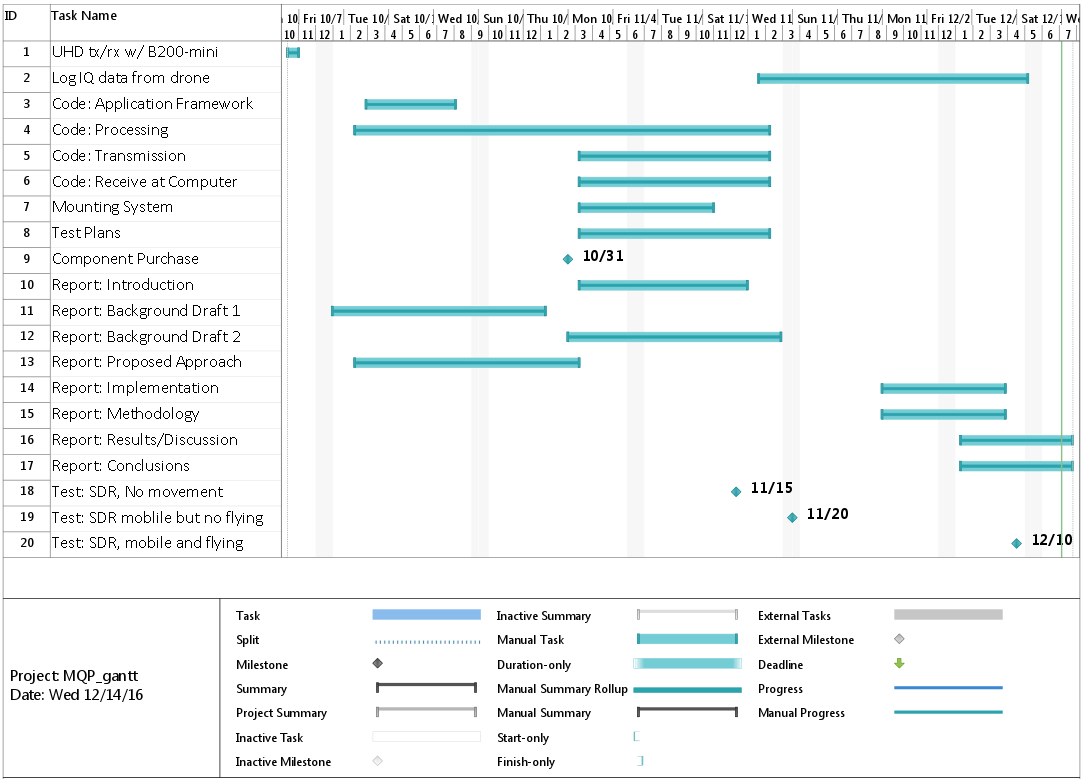
\includegraphics[width=1.0\textwidth]{img/oct_gantt_chart.png}
\caption{Project Planning Gantt Chart}
\label{fig:gantt_chart}
\end{figure}
